\documentclass[tikz]{standalone}
\usepackage{framed}
\usepackage{amsmath} 
\usepackage{amsfonts}
\DeclareMathOperator{\f}{f}
\usepackage{xcolor}

\usetikzlibrary{shadows.blur}
\usetikzlibrary{arrows}
\usetikzlibrary{positioning}

\begin{document}
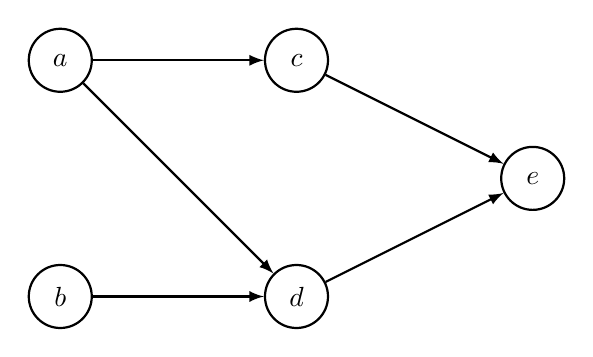
\begin{tikzpicture}[]
	%\draw[help lines] (-2,0) grid (20,10);
	
	\tikzstyle{vnode} = [circle,draw,thick,fill=white,minimum size=8mm]
	\tikzstyle{vedge} = [->,>=latex,thick]
	
	\node[vnode] (a) at (-9,0.5) {$a$};
	\node[vnode] (b) at (-9,-2.5) {$b$};
	\node[vnode] (c) at (-6,0.5) {$c$};
	\node[vnode] (d) at (-6,-2.5) {$d$};
	\node[vnode] (e) at (-3,-1) {$e$};
	
	\draw (a) edge [vedge] (c);
	\draw (a) edge [vedge] (d);
	\draw (b) edge [vedge] (d);
	\draw (c) edge [vedge] (e);
	\draw (d) edge [vedge] (e);

\end{tikzpicture}
\end{document}
